% THIS IS SIGPROC-SP.TEX - VERSION 3.1
% WORKS WITH V3.2SP OF ACM_PROC_ARTICLE-SP.CLS
% APRIL 2009
%
% It is an example file showing how to use the 'acm_proc_article-sp.cls' V3.2SP
% LaTeX2e document class file for Conference Proceedings submissions.
% ----------------------------------------------------------------------------------------------------------------
% This .tex file (and associated .cls V3.2SP) *DOES NOT* produce:
%       1) The Permission Statement
%       2) The Conference (location) Info information
%       3) The Copyright Line with ACM data
%       4) Page numbering
% ---------------------------------------------------------------------------------------------------------------
% It is an example which *does* use the .bib file (from which the .bbl file
% is produced).
% REMEMBER HOWEVER: After having produced the .bbl file,
% and prior to final submission,
% you need to 'insert'  your .bbl file into your source .tex file so as to provide
% ONE 'self-contained' source file.
%
% Questions regarding SIGS should be sent to
% Adrienne Griscti ---> griscti@acm.org
%
% Questions/suggestions regarding the guidelines, .tex and .cls files, etc. to
% Gerald Murray ---> murray@hq.acm.org
%
% For tracking purposes - this is V3.1SP - APRIL 2009

\documentclass{acm_proc_article-sp}
\usepackage{float}
\usepackage[]{graphicx,subfigure}
\usepackage{verbatim,color}

\begin{document}

\title{Large Data and Computation in a Hazard Map Workflow Using Hadoop and Neteeza Architectures}
%\subtitle{[Extended Abstract]}
%\titlenote{A full version of this paper is available as
%\textit{Author's Guide to Preparing ACM SIG Proceedings Using
%\LaTeX$2_\epsilon$\ and BibTeX} at
%\texttt{www.acm.org/eaddress.htm}}}
%
% You need the command \numberofauthors to handle the 'placement
% and alignment' of the authors beneath the title.
%
% For aesthetic reasons, we recommend 'three authors at a time'
% i.e. three 'name/affiliation blocks' be placed beneath the title.
%
% NOTE: You are NOT restricted in how many 'rows' of
% "name/affiliations" may appear. We just ask that you restrict
% the number of 'columns' to three.
%
% Because of the available 'opening page real-estate'
% we ask you to refrain from putting more than six authors
% (two rows with three columns) beneath the article title.
% More than six makes the first-page appear very cluttered indeed.
%
% Use the \alignauthor commands to handle the names
% and affiliations for an 'aesthetic maximum' of six authors.
% Add names, affiliations, addresses for
% the seventh etc. author(s) as the argument for the
% \additionalauthors command.
% These 'additional authors' will be output/set for you
% without further effort on your part as the last section in
% the body of your article BEFORE References or any Appendices.

\numberofauthors{3} %  in this sample file, there are a *total*
% of EIGHT authors. SIX appear on the 'first-page' (for formatting
% reasons) and the remaining two appear in the \additionalauthors section.
%
\author{
% You can go ahead and credit any number of authors here,
% e.g. one 'row of three' or two rows (consisting of one row of three
% and a second row of one, two or three).
%
% The command \alignauthor (no curly braces needed) should
% precede each author name, affiliation/snail-mail address and
% e-mail address. Additionally, tag each line of
% affiliation/address with \affaddr, and tag the
% e-mail address with \email.
%
% 1st. author
\alignauthor
Shivaswamy Rohit\\
       \affaddr{Dept. of Mechanical and Aerospace Engineering}\\
       \affaddr{University at Buffalo}\\
       \affaddr{New York, USA}\\
       \email{shivaswa@buffalo.edu}
% 2nd. author
\alignauthor
Abani K. Patra \\
       \affaddr{Dept. of Mechanical and Aerospace Engineering}\\
  \affaddr{University at Buffalo}\\
       \affaddr{New York, USA}\\
       \email{abani@buffalo.edu}
% 3rd. author
\alignauthor Vipin Chaudhary \\
       \affaddr{Dept of Computer Science and Engineering}\\
  \affaddr{University at Buffalo}\\
       \affaddr{New York, USA}\\
       \email{vipin@buffalo.edu}
}
% There's nothing stopping you putting the seventh, eighth, etc.
% author on the opening page (as the 'third row') but we ask,
% for aesthetic reasons that you place these 'additional authors'
% in the \additional authors block, viz.
%\additionalauthors{Additional authors: John Smith (The Th{\o}rv{\"a}ld Group,
%email: {\texttt{jsmith@affiliation.org}}) and Julius P.~Kumquat
%(The Kumquat Consortium, email: {\texttt{jpkumquat@consortium.net}}).}
%\date{30 July 1999}
%% Just remember to make sure that the TOTAL number of authors
% is the number that will appear on the first page PLUS the
% number that will appear in the \additionalauthors section.

\maketitle

% A category with the (minimum) three required fields
%\category{H.4}{Information Systems Applications}{Workflow management}
%A category including the fourth, optional field follows...
%\category{H.2.8}{Database Applications}{Scientific databases }

%\terms{Theory}

\keywords{Uncertainty Quantification, Data Warehouse Appliance, Hadoop} % NOT required for Proceedings

\input{discs_intro}

\begin{comment}

\begin{figure*}
\begin{center}
\subfigure{
\resizebox*{10cm}{!}{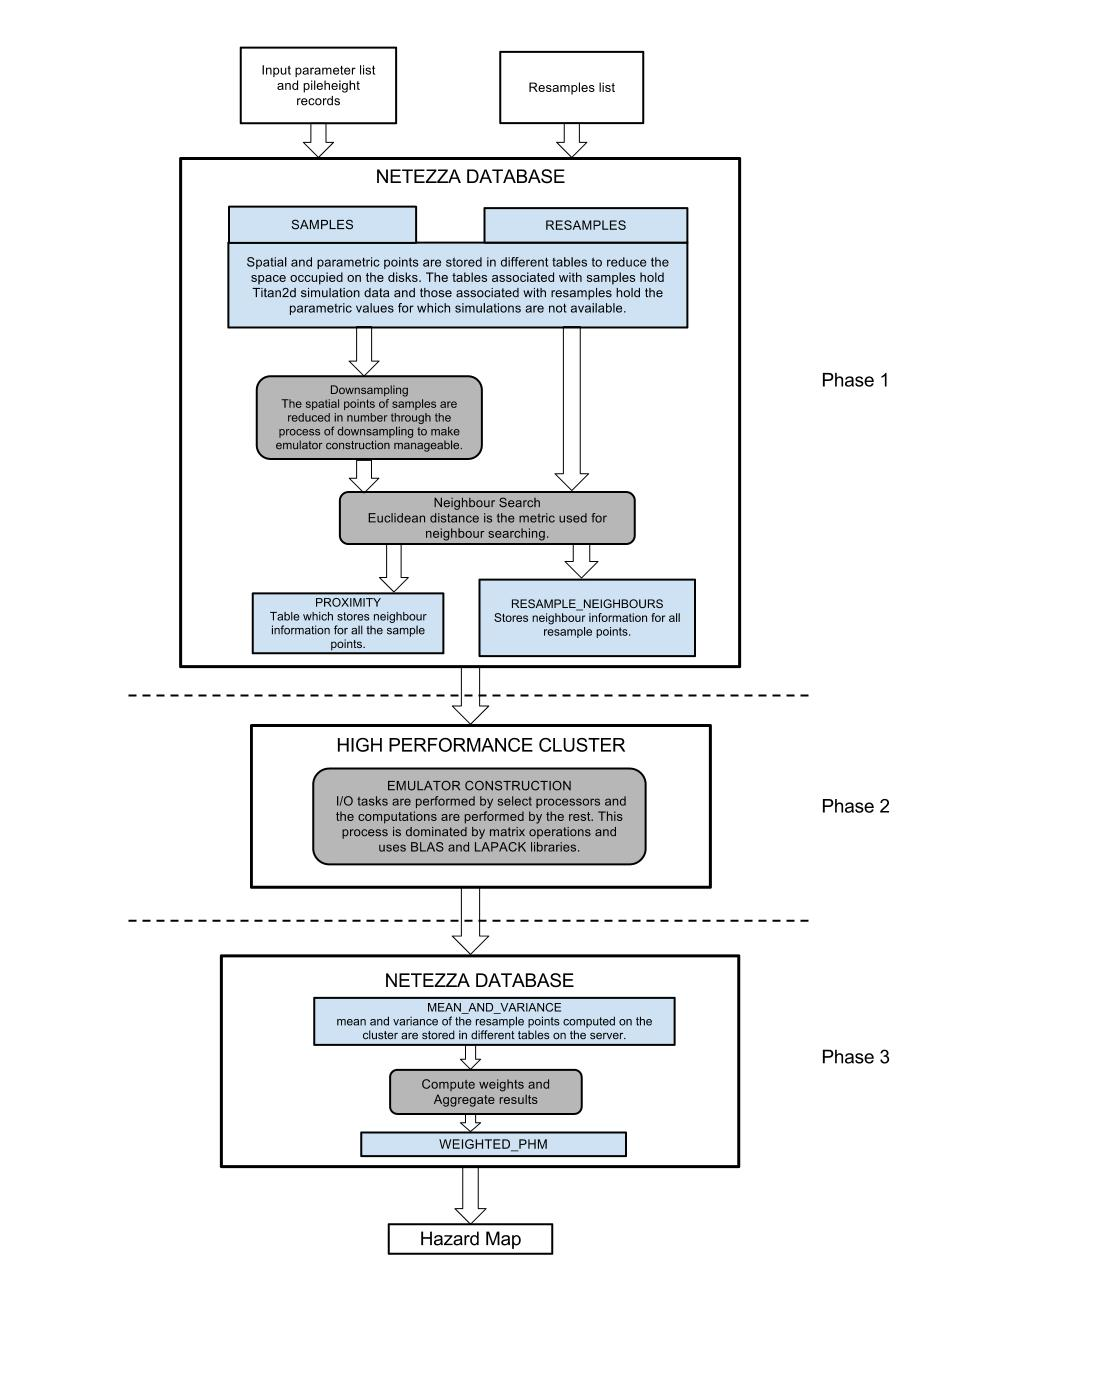
\includegraphics{Workflow2.jpg}}}%
\subfigure{
\resizebox*{10.4cm}{!}{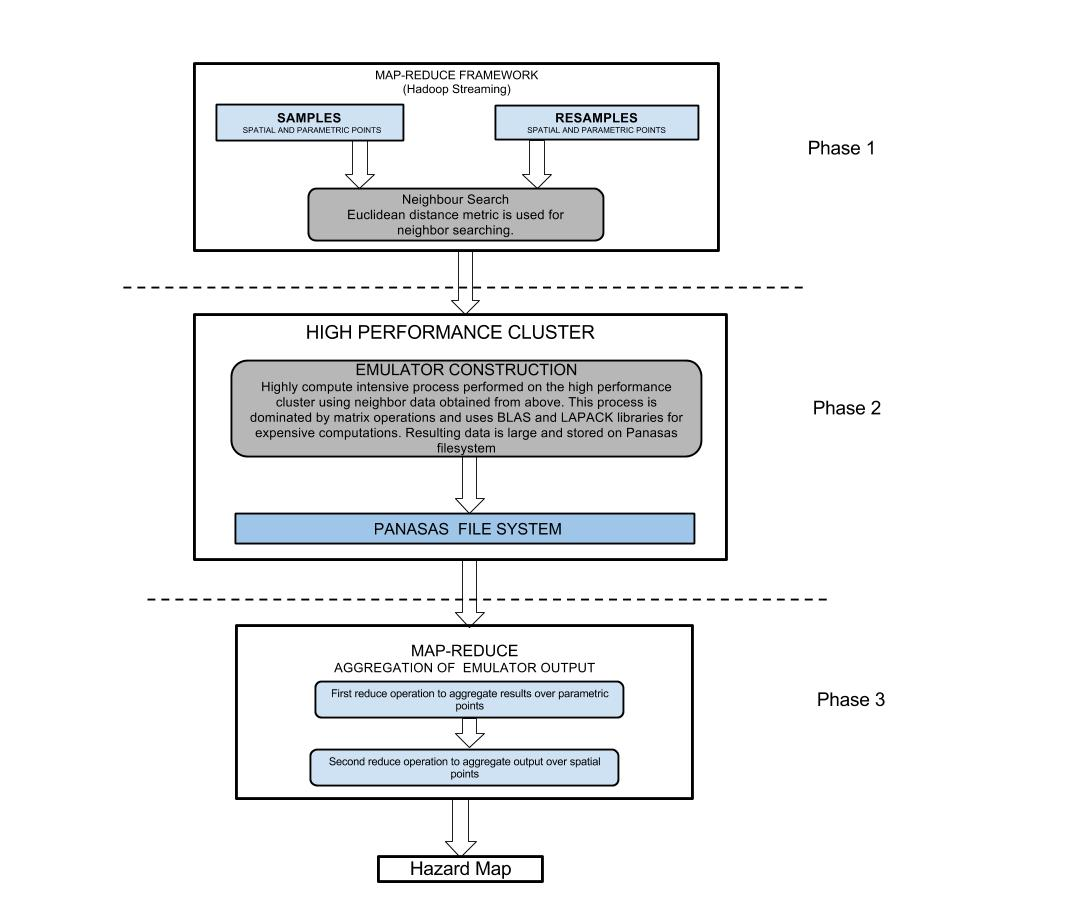
\includegraphics{Hadoop_Workflow.jpg}}}%
\caption {Figure shows the probabilistic hazard map for the island of Montserrat in the Caribbean for flow exceeding 0.2m of depth.} \label{map2}
\end{center}
\end{figure*}
\end{comment}


\section{ Hazard Map Generation --  Data Management and Computing}\label{HMG}
%Constructing and using the emulator entails with it not only a computationally challenging task but also the burden of storing,
%manipulating and moving massive
%amount of data. 
%Also the size of data changes significantly during the process.
To understand the complexity of the problem
we present an outline of steps involved in a usual process of Hazard map generation.\\

\begin{enumerate}
\vspace{-0.2in}
\item [ {\bf Step 0:}] The first step is to run the simulator at well chosen inputs. The input parameters
%sample the parameters, to construct the emulator.
%which include but are not limited to the initial volume of pile, 2 parameters of
%location, and the internal friction, 
are sampled using a simple space filling design like Latin Hypercube to obtain  2048 sets of input.
Multiprocessor Titan2D  simulations of these inputs  and post processing results in 
2 gigabytes(GB) of flowdata per sample in the form of flow height records. 
%The input parameters along with spatial co-ordinates of the flow account 
%for all the random variables considered to induce uncertainty in the system.
\item [ {\bf Step 1:}] { The construction of the hazard map requires us to sample a tensor product of the input parameters and 2 space dimensions
which results in as many as 10$^{8}$ data points. Emulator construction on this very large set is unaffordable so a simple 
contouring and decimation strategy is used to create a smaller set on which we construct the emulator.
This 
downsampling is introduced to reduce their number to the order of 10$^{6}$. Furthermore, 
resamples from the generated emulator surface (for the final probability calculation) are also required to be generated and can be as many as $10^{10}$ in number.}

\item [ {\bf Step 2:}]The size of the downsized  data set makes it computationally impossible to fit a single emulator using all the data 
at once, which warrants the need for piecewise emulator obtained by localizing the covariance. The
neighbor search used in identifying the regions for localization is thus an important pre-requisite for the functioning of the
emulator and requires both sample and resamples to be searched from among the samples for neighbors. Both neighbor search and downsampling
are highly data intensive tasks which require little computation but scanning of large datasets.

\begin{figure}
\begin{center}
%\resizebox*{15cm}{!}{\includegraphics{net_flow.pdf}}
\resizebox*{10cm}{!}{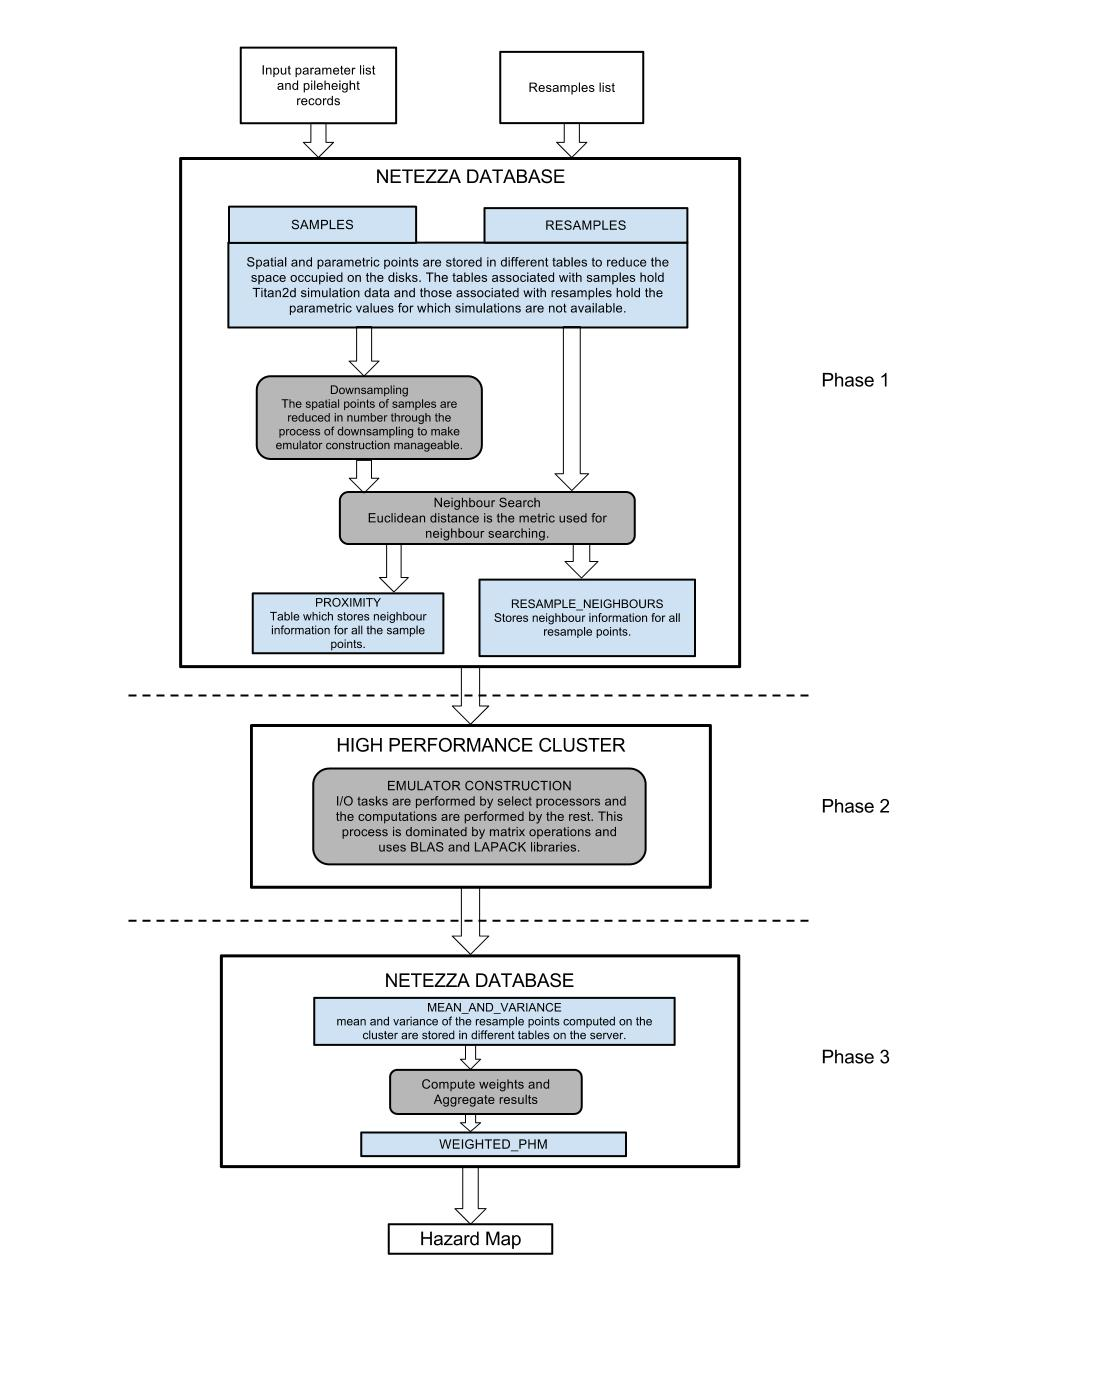
\includegraphics{Workflow2.jpg}}
\vspace{-40pt}
\caption{\label{fig2} Illustration of the integrated workflow using Netezza architecture.}%
\end{center}
\end{figure}

\begin{figure}
\begin{center}
%\resizebox*{15cm}{!}{\includegraphics{net_flow.pdf}}
\resizebox*{10cm}{!}{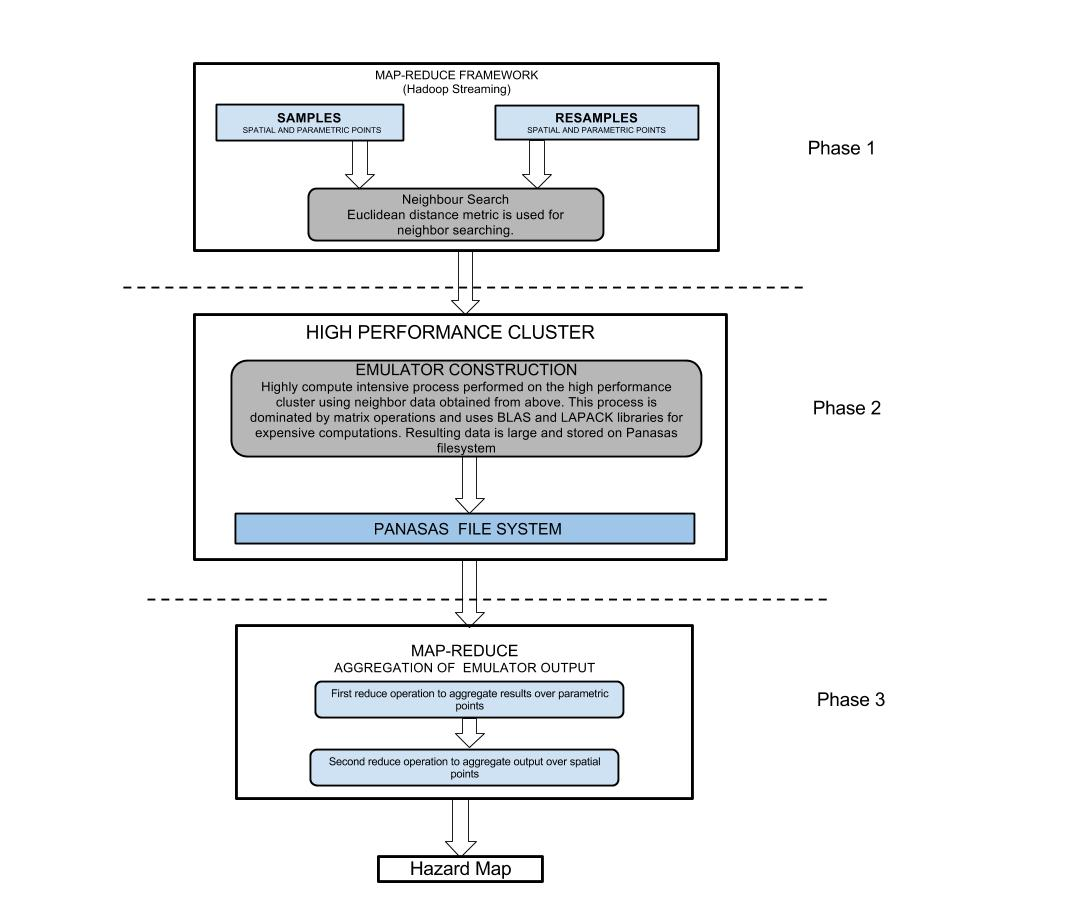
\includegraphics{Hadoop_Workflow.jpg}}
\vspace{-25pt}
\caption{\label{fig2} Illustration of the integrated workflow with Map-Reduce framework}
\end{center}
\end{figure}



\item [ {\bf Step 3:}] Using neighborhood data, emulator is constructed about the sample points through an iterative process. 
The functioning of emulator can be understood from the following equations:
%by superimposing equations \ref{mean} and \ref{reg} which yields

\begin{subequations}\label{mean1}
\begin{equation}
                                E(s(y)|s(x)) = g(y)\beta + {r(y)}^{T}{R}^{-1}\epsilon
\end{equation}
\begin{equation}
                                Var[s(y)|s(x)] = {\sigma}^{2}(1 - {r(y)}^{T}{R}^{-1}r(y))
\end{equation}
\end{subequations}
\begin{equation}
                                r_{i}(y) = exp\left(-\sum_{n=1}^{N_{dim}} \theta_n(y_n-x_{i,n})^{2}\right)
\end{equation}


g(y) being  the matrix of basis functions evaluated at the resample points and $\beta$ being the vector of least square co-efficients.
R is the matrix of the correlation functions at x such that R$_{i,j}$ = r$_{i}$(x$_{j}$) = r$_{j}$(y$_{i}$) and $\sigma$ is the variance.

%Equation \ref{mean1}(a) clearly indicates that the emulator is composed of a mean which is approximated using least square fit, and an error term
%which is modeled as a gaussian process with 

$s(x) = {\beta}G(x) + \hat{\epsilon}$ is the response function.

$\epsilon$ = s(x) - G(x)$\beta$ the true error evaluated at the sample points. 
$\theta$$_{n}$ is the
vector of hyper-parameters or roughness parameters and Ndim is the number of dimensions associated with the data set.


At each iteration 
$\beta$ and R$^{-1}$ are computed using updated values of hyper-parameters ($\theta$).
%The emulator is set up using the data from the neighborhood of the point about
%which it is constructed. A covariance matrix (required for the gaussian error model) has to be set up and its inverse computed through an iterative
%procedure to ascertain the correct correlation lengths.
Mean and variance are then evaluated for the resamples and adjusted using bayes
linear equations. Typically, a hazard map requires constructing a few million emulators.
The emulator construction dominated by O($n^{3}$) matrix operations is a highly compute intensive process but also embarrassingly
parallel.

\item [ {\bf Step 4:}] In the last stage of hazard map construction, emulator output is aggregated using barycentric weights.
This involves scanning the dataset, computing the euclidean distance of the samples that influence a resample point, evaluating their weights
 and assembling the results.

\end{enumerate}



\section{Integrated Workflow for data and compute intensive tasks}
%It is clear from section \ref{HMG} that 
There are three dominant phases of Hazard Map generation namely:
1) Downsampling and neighbor searching,
2) Emulator construction, and, 3)Aggregation of resulting data.
Our computational model based on a $\it{divide}$ $\it{and}$ $\it{conquer}$ strategy, segregates these phases and performs them on either Netezza
server or the high performance cluster depending on the computational requirements.

\subsection{Downsampling and neighbor search}
%Both downsampling and neighbor search are ideally suited to be performed on the Netezza database.
Both downsampling and neighbor search are ideally suited for distributed systems.
For multidimensional dataset, such as ours, operations like neighbor search are afflicted with the $\textit{curse of
dimensionality}$. Several tree and clustering based methods have been proposed but most converge to sequential search for higher dimensions
and/or are difficult to implement. Neighbor search operation 
on a distributed environment like Netezza server or on a cluster through Map-Reduce
implementation like Hadoop allows for a much simpler algorithm and adapts to large datasets.
Downsampling and Neighbor search on the Netezza system were easily accomplished because of its massively parallel architecture.
%Downsampling on the Netezza system required a single query applied to the entire dataset of pileheight records which
%selects points at regular intervals on the grid. 
%Previous implementation of this on HPC platforms were significantly complex \cite{keith}.
Netezza's high performance stems from filtering data close to disk and from its MPP architecture. Since a significant amount of data
movement is curtailed through the use of FPGA filtering, we abstained from using complex algorithms in favor of brute force
techniques. All Netezza based implementations were in plain SQL which ensured parallelism and high performance. 

We also tested same operations on the high performance cluster using python scripts, relying on Hadoop Streaming API for 
task distribution and scheduling. 
In a distributed environment the  underlying algorithm for neighbor search remains essentially the same as the
one used on Netezza server. The mapper  computes the distances between two sets of data (X and Y) and prints out the result as key-value
pair, key being the indices of dataset X and value being the indices of dataset Y  and the euclidean distance. 
In the absence of a customized partitioner
same keys are guaranteed to be dispatched to the same reduce task. The reduce operation merely involves printing out the indices of set Y
against the keys obtained from set X. Hadoop based implementation as in the case with Netezza was simple and concise.

In both our implementations euclidean distance was the metric for neighbor search.
The parametric neighbor search was performed independent of spatial neighbor search by
separately treating the two sets of dimensions. 
Though the brute force method of neighbor search has a complexity of O($n^{2}$), it is well suited for distributed environment
owing to good scalability.

\begin{comment}
the Netezza
architecture is ideally suited for such methods.  The distance based neighbor search also made it possible to more
precisely define the region of neighborhood which could not have been achieved using tessellation based neighbor search. A notable advantage
of neighbor search on the database is that it can be easily extended to even higher dimensions without the need of any significant changes in
the implementation.\\

Database operations played a pivotal role in our computing model by making the cumbersome task of data-mining on the cluster a rather elegant
and transparent process. Netezza's datawarehousing capabilities ensured that all data could be stored at one place as opposed to having it
scattered across a
large number of flat files on the cluster. Using SQL, clean and concise codes could be written with provision for easily making changes.
Several hundreds of lines of MATLAB code were replaced with less than hundred SQL queries. Data warehousing capability and ``under the hood" data
movement offered an enormous respite from the MATLAB implementation on the cluster where data movement was achieved by reading and writing of a
large number ASCII files. Table \ref{tables} lists some of the tables that were generated on Netezza for one of the cases prior to emulator
construction. Tables with rows of the order of millions and even close to 2 billion in case of table $\small{PROXIMITY}$ were generated with
ease.\\
\end{comment}


\begin{comment}
\begin{table*}
\centering
\caption{Some Typical Commands}
\begin{tabular}{|c|c|c|} \hline
%Command&A Number&Comments\\ \hline
\bf{Table Name} & \bf{Number of rows} & \bf{Description}\\ 
Titan & 149,207,040 & Pileheight and spatial co-ordinates of all the sample points.\\ \hline
Downsampled &  4,054,229 & Points retained after downsampling.\\ \hline
Samples\_Scaled & 2048 & Input parameters used for simulation.\\ \hline
Resamples & 99,304 & Input parameters for which simulation data is not available.\\ \hline
Uniq\_Coord & 10,068 & Indices of unique points on the grid pertaining to downsampled data.\\ \hline
Proximity & 1,903,673,287 & neighbors of every downsampled point.\\ \hline
Macro\_neighbor & 214054 & neighbors of input parameters.\\ \hline
Phm\_neighbors & 226,691,049 & neighbors of spatial points of resamples\\ \hline
Resample\_neighbors & 466858 & neighbors of input parameters of resamples from the samples.\\ \hline
%\texttt{{\char'134}alignauthor} & 100& Author alignment\\ \hline
%\texttt{{\char'134}numberofauthors}& 200& Author enumeration\\ \hline
%\texttt{{\char'134}table}& 300 & For tables\\ \hline
%\texttt{{\char'134}table*}& 400& For wider tables\\ \hline
\end{tabular}
\end{table*}
\end{comment}






%With the data mining operations successfully accomplished, all the information required for emulator construction was available for immediate
%use in the form of tables on Netezza database.
% However, unlike the computations up to this point, the emulator construction is a
%computationally expensive process involving large number of matrix operations. 

%For a 
%By performing a few simple tests it was clear that Netezza was
%not well suited for emulator construction.
% Since the emulator construction is dominated by matrix operations 
%We attempted large number
%of matrix multiplication operations on Netezza using SQL and deduced that emulator construction on the database 
%would not be feasible under a reasonable time frame.
 %Table \ref{mat} %shows the time taken for performing multiplication on matrices of size 200x200. 
%Figure \ref{mulplot} shows an almost linear dependence between the number of matrix multiplication operations for square matrices of size
%200x200 and the time taken. An extrapolation of this data yields the time taken for 4 million operations at approximately 7 hours. In practice,
%linear dependence would not extend over such large number of operations owing to limited memory on S-blades. Also the number of matrix
%operations is much larger than 4 million.\\



%\subsection{Integrating Netezza with High Performance Cluster}
\subsection{Emulator Construction}
Unlike the data mining operations up to this point, the emulator construction is a computationally expensive process dominated by 
matrix operations. Though emulator conctruction is an embarrassingly parallel process and Netezza server boasts of massively 
parallel architecture, it was, for variety of reasons as we describe below,
appropriate to siphon data off
the database to an architecture that could meet the emulator's computational demands. First, complex algorithms can not be easily translated
into a declarative language like SQL. Second, the number of blades available in our systems put a limit on the available processors. Also the
explicit use of high performance libraries like \textit{blas} and \textit{lapack} was not possible. Another subtle aspect
about emulator which advocates against its construction on the database is that it requires small chunks of data, more precisely the
neighborhood data. Netezza is  more appropriate for scanning large datasets. We present here the steps taken and the challenges faced in 
integrating server to the cluster.

The high performance cluster and the Netezza system were connected using Netezza's
ODBC driver. Data transfer across the two frameworks was possible largely through the use of named pipes. On linux systems a
named pipe is a type of file - FIFO file (FIFO being the acronym for First In First Out). A named pipe does not store or buffer data and
hence does not occupy storage space on the filesystem.\\
Loading data from cluster to Netezza was achieved through the \textit{nzload} feature. The \textit{nzload} command is a SQL CLI client
application which in conjunction with named pipes that makes it possible to load data 
to Netezza server from any remote client\cite{data_load}. 
%Use of nzload together with named
%pipes greatly simplified transfer of data. The nzload command makes direct insertions to the target table, and the transaction is committed on
%closing the pipe. Multiple instances of nzload, can simultaneously load data on the server in  parallel.\\

\begin{figure}
\begin{center}
\resizebox*{8cm}{!}{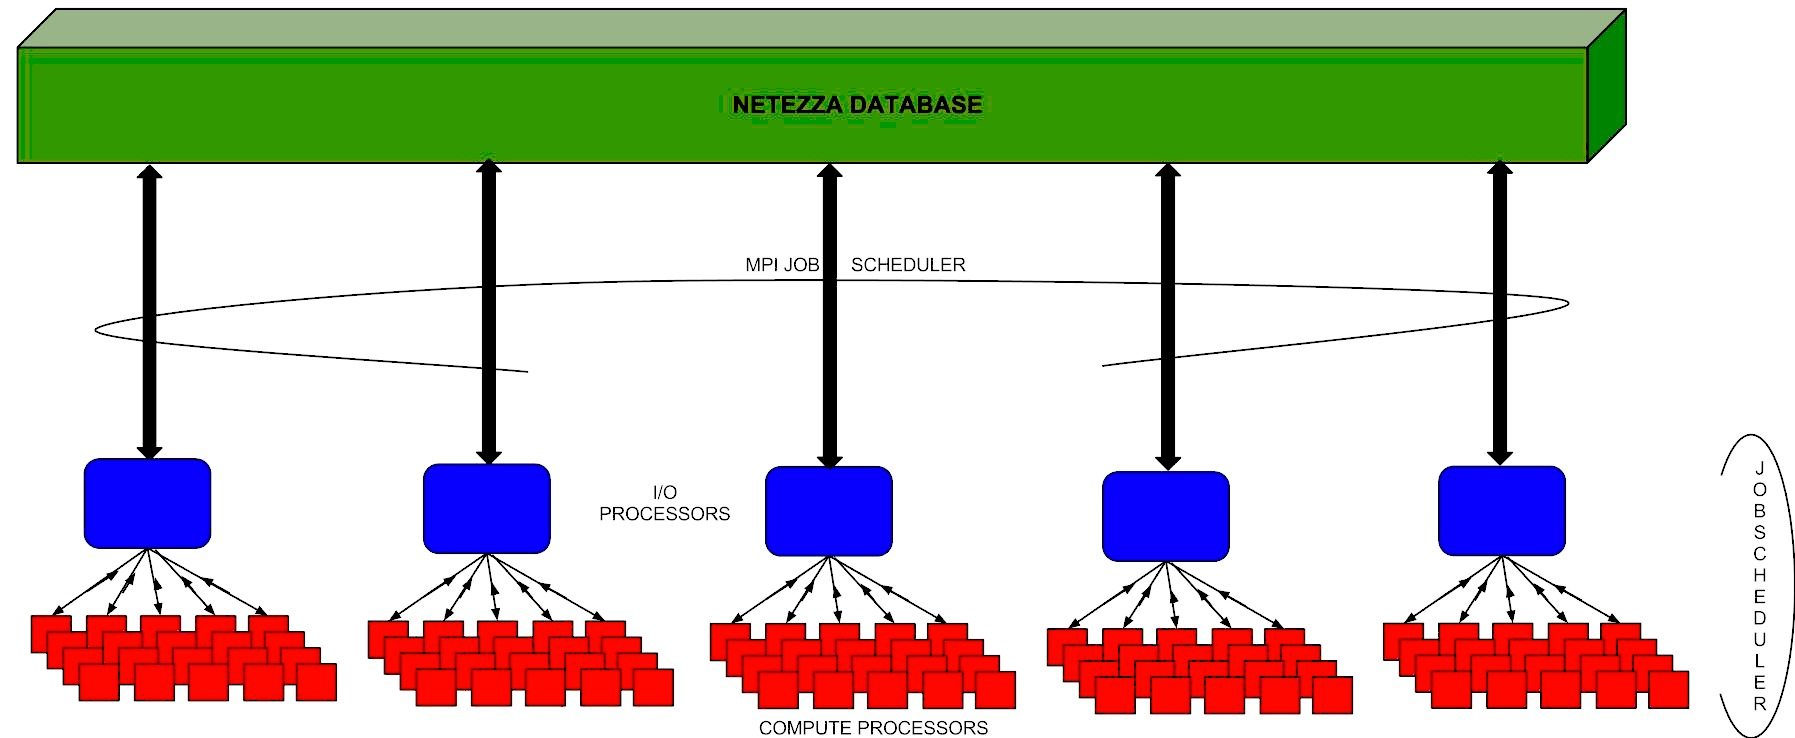
\includegraphics{cluster.jpg}}
\caption{\label{fig2} Schematic representation of integration of Netezza with high performance cluster}%
\end{center}
\end{figure}


\begin{figure*}
\begin{center}
\subfigure{
\resizebox*{7cm}{!}{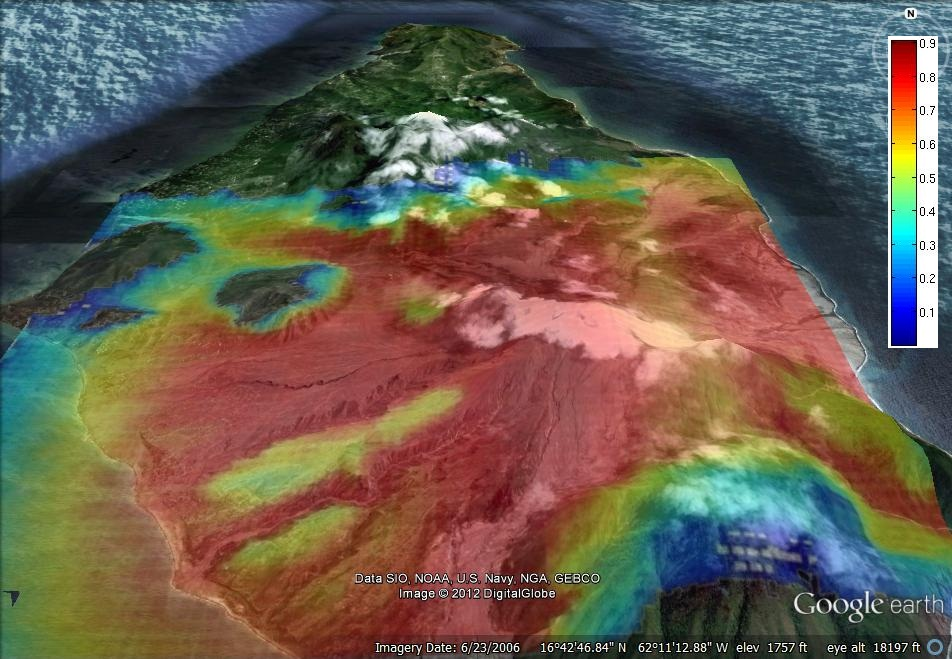
\includegraphics{new_map_colorbar.jpg}}}%
\subfigure{
\resizebox*{7.4cm}{!}{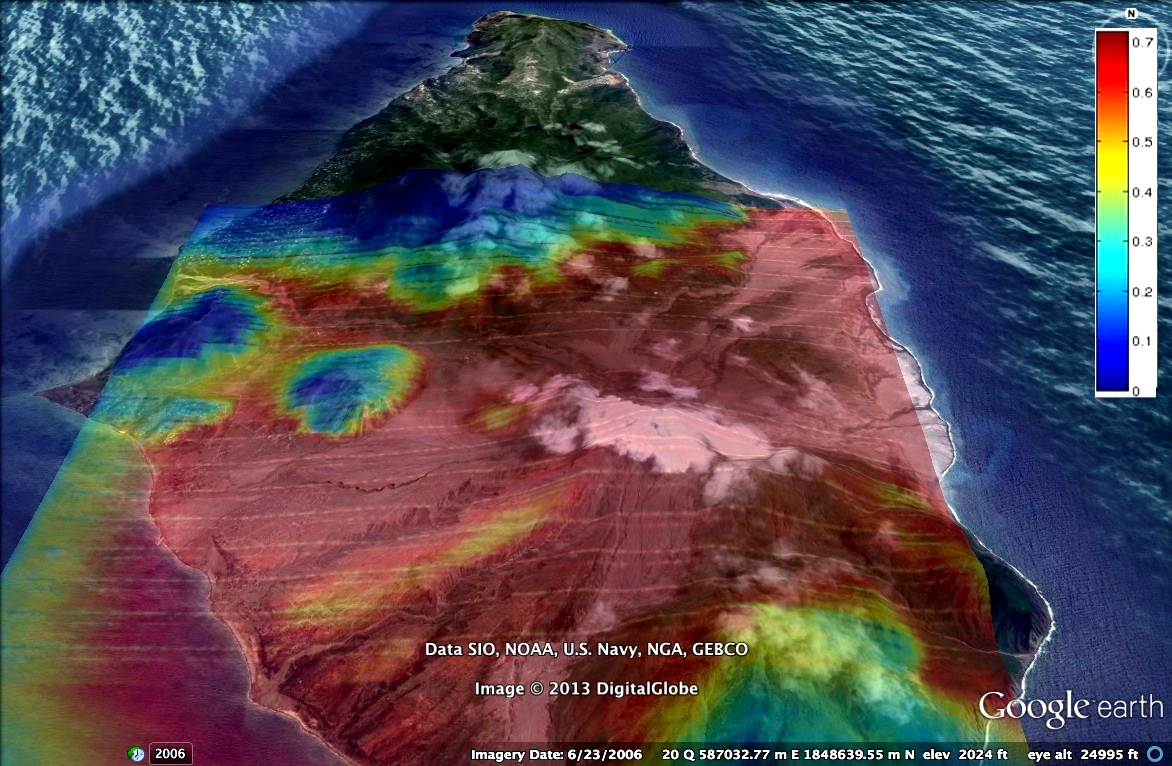
\includegraphics{Hadoop_map.jpg}}}%
\caption {Figure shows the probabilistic hazard maps for the island of Montserrat in the Caribbean for flow exceeding 0.2m of depth.
One on left was generated using Netezza database based model and the one on right using Hadoop API} \label{map2}
\label{maps}
\end{center}
\end{figure*}


Emulator construction requires that each processor request the server for its share of data. Large number of concurrent I/O requests by nodes
on the grid can result in I/O bottlenecks and processors starving for data. Such problems have been addressed in the past and techniques such
as collective I/O\cite{cite4,kotz} and I/O forwarding\cite{cite5} have been proposed. I/O forwarding mitigates this problem by passing the I/O
requests of the all the nodes to only a select number of nodes called as I/O nodes. We adopted this method for our computing model with some
modifications.\\
A few processors on the high performance cluster are identified as the I/O processors and the rest as compute processors. All the processors
are assigned a group, with each group having one I/O processor and several compute processors. Each group operates independent of the other
with I/O processors responsible for performing all I/O operations on behalf of the compute processors of their respective groups. I/O
processors alone communicate with the Netezza server and any transfer of data occurs through named pipes. Multiple small requests are avoided
and data is invariably transferred in bulk. I/O processors extract data from Netezza, disseminate it across the compute processors and deliver
the data gathered from the compute processors back to the Netezza database. I/O processors of every group draw the neighborhood data of all
the downsampled points corresponding to the pileheight simulation number assigned to them from sever, and store it in their data structures.
Each compute processor based on the data received from the I/O processor of its group builds an emulator. The mean and variance data of the
resample points, computed at the end is sent over the network to I/O processor.\\
The operations on the cluster are parallelized using MPI (Message Passing Interface). Data is transferred between the I/O and compute processors
over the network using MPI protocols. An MPI job scheduler allows compute processors to notify the I/O processors about the status of their
completion. When a compute processor finishes constructing emulator about a sample point, it prompts the I/O processor. The I/O processor
responds by sending neighborhood data for the next point. The compute processors do not communicate among themselves and are self sufficient
with the data received from the I/O processor. The mean and variance information received from the compute processors is allowed to accumulate
with I/O processors and dispatched to the Netezza server at regular intervals. Another layer of MPI job-scheduler is responsible for
co-ordination between the various groups of processors. A lone processor which holds the metadata maintains communication with the groups and
assigns each group a simulation number to work on. Additionally it also prompts Netezza database to ``generate statistics" after each load
session.

Though we succeeded in integrating server with the cluster and in transferring data over the network, this implementation has apparent
shortcomings. Firstly offloading compute intensive tasks from server to cluster defeats the objective of minimizing large data movement.
Secondly only a small number of ports can be kept working between the two, to transfer data. Thus, though Netezza can easily house much
more data, extracting it to more nodes on cluster is not feasible. It is thus clear that compute intensive tasks like emulator construction
expose the vulnerabilities of even a specialized hardware like Netezza database. For the above mentioned reasons and also because of the 
complexity of implementation,  we attempted to test the above model with Hadoop in place of Netezza. Hadoop provides a convenient alternative
because it does not require data to be moved into or out of the cluster. The downsampled points stored on files on the Hadoop distributed
file system were used as input to the mapper. The mapper itself was simply a python wrapper around the existing code to compute the emulator
with output in terms of key value pairs. 
Hadoop is designed to take in large amount of input and distribute the tasks by spawning mappers on each of the slave nodes. In our application
at less than 2GB the input data was very insignificant in size but the generated output was expected to be large. Also the emulator construction
is highly cpu intensive. 
We observed that no more than 2 map tasks could be spawned on each node regardless of the number of cores on them.
On certain nodes, with say 12 cores, having only 2 map tasks running was a severe under utilization of the resources.
Also, previous experience dictates that at least 500 processors be used for emulator construction to finish the 
hazard map in reasonable time. Under these circumstances we found it to be more appropriate to perform emulator construction independent
of Hadoop environment. The resulting output was stored as key-value pairs on ASCII files. 





\subsection{Aggregation Of Results}
The first two moments are to be computed for every resample point, which as mentioned 
earlier, could be as many as $10^{10}$ in number. Furthermore most of these points occur in the neighborhood of more than one sample point. In
the previous work \cite{keith}, the weights were pre-computed owing to the fixed number of neighbors which made immediate aggregation of data
possible. A distance based method of neighbor search is computationally more expensive. The

Netezza database offers aggregate functions and can easily house massive data. The "group by" feature of any database is primarily aimed at
operations like reduction and aggregation. Besides, computing the
 weights required repeated scanning of large parts of the data sets.
Netezza is well suited for such aggregation of data.  The mean and variance computed by the compute processors is directed
to the Netezza server through the I/O processors. The cluster and the Netezza server are connected by 10Gb network at the Center for
Computational Research, Buffalo. Using Netezza's nzload command and with multiple named pipes, data is concurrently moved from I/O processors
to the respective tables on Netezza. The mean and variance data is massive and runs into billions of rows on the server. 
It is important that
the tables storing such data are already distributed on columns on which they are aggregated. This ensures prior partitioning of data about
those columns which significantly reduces the computation time. During the implementation of certain aggregation queries we found, that by
having the table (with approximately 2 billion rows) distributed on the columns to be aggregated on, the total time of operation was reduced
from approximately 30 minutes to under 3 minutes.



A Hadoop based aggregation of the emulator output was performed by chaining of map-reduce operations. As the term suggests,
aggregation, did not require any specific map operation. As the output was required to be aggregated over 
multiple set of keys, aggregation was split into two separate reduce operations. 
Both the tasks involved only stdin and stdout operation in the mapper. The reducer was responsible for assembling the weighted mean 
for records with same keys. The replication factor was fixed at 1 for Hadoop implementations.




%%%%%%%%%%%%%%%%%%%%%%%%%%%%%%%  BEGIN COMMENTS  %%%%%%%%%%%%%%%%%%%
\begin{comment}
\begin{figure}[H]
\begin{center}
%\subfigure{
%\resizebox*{6cm}{!}{\includegraphics{noflow.jpg}}}%
\subfigure{
\resizebox*{6cm}{!}{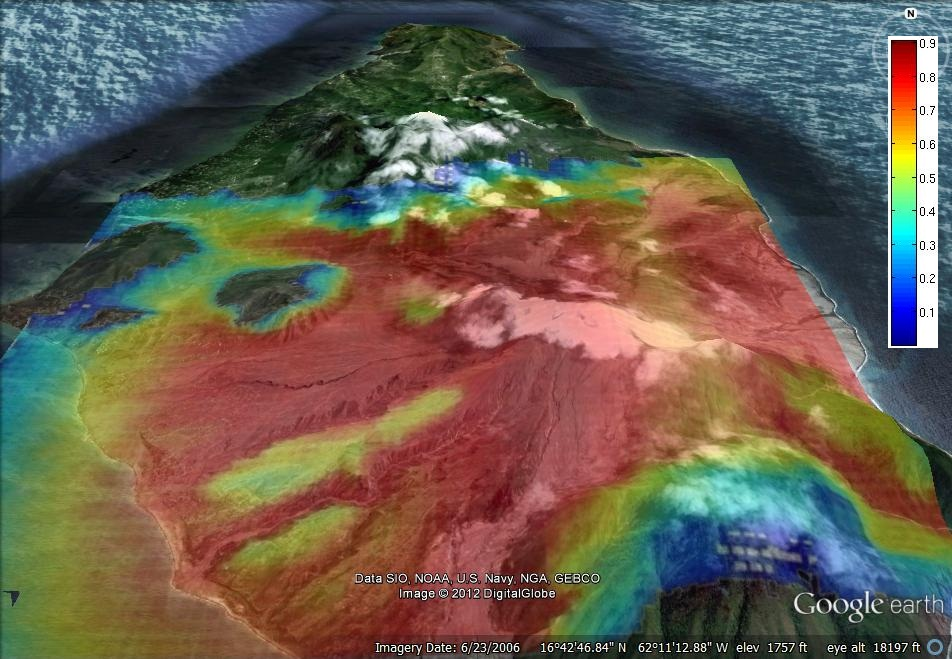
\includegraphics{new_map_colorbar.jpg}}}%
\caption {Figure shows the probabilistic hazard map for the island of Montserrat in the Caribbean for flow exceeding 0.2m of depth.} \label{map2}
\end{center}
\end{figure}

The resulting 2048 pileheight records 
were merged using python
scripts and loaded on the Netezza server for downsampling and neighbor searching. The details of some of the tables generated are already provided
in Table 1. The dimensions associated with the random
variables being vastly different and having very different scales, were all mapped to the same scale of 0 to 1. Matrix operations being
expensive, it was essential to keep their sizes small. Thus a limit on the number of neighbors had to be
enforced in addition to a limit on the euclidean distance.

The computational details of the hazard map shown in figure \ref{maps}are enumerated below.
\begin{enumerate}
{
\item The Hazard map was generated using the our computational model comprising of the Netezza server and
504 processors on the high performance cluster.
\item Neighbor search, downsampling and few other operations were performed on Netezza in 30 minutes. The radius of neighborhood was fixed at 
0.3 for parametric dimensions
(scaled) and 200 metres for spatial dimensions. Furthermore, each sample point could have at most 500 neighbors and this
information was stored in the table $\small{PROXIMITY}$.
\item 504 processors functioning as 18 independent groups were responsible for emulator construction and the evaluation of mean and variance
using Bayes Linear model. Each group had 1 I/O processor and at most 27 compute processors.
\item During 8 hours 47 minutes of wall time on the cluster, approximately 4 million covariance matrices of size 300x300 were computed
through an iterative process and mean and variance was computed for approximately $10^{10}$ resample points.
\item In that time more than 1.5 TB of data was transferred over the network to Netezza server over 18 different pipes. 
This data was stored on 18 different tables occupying a little more than a total of 50 billion rows.
\item The final step which required scanning billions or rows of data to evaluate the barycentric weights and aggregate the results
was also performed on the Netezza server and took 2.5 hours of time.
\item The entire operation completed in little under 12 hours of time.\\
}
\end{enumerate}
\end{comment}
%%%%%%%%%%%%%%%%%%%%%%%%%%%%%%%% END  OF COMMENTS  %%%%%%%%%%%%%%%%%%%%%%%%%%%%%%%%%%%%%%%%%%%%%%%%%%%%%%%%%%%%%%%%%%

\section{Results}
We put both computing models was put to test with the task of creating the hazard map for the volcano on Montserrat island. 
2048 sets of input parameters were generated using Latin Hypercube sampling and Titan2D simulations of these inputs were performed. 
The probabilistic hazard map shown on the left in figure \ref{map2} was generated, 
%with the same input parameters and with above modifications
%incorporated in the code, 
in 6 hours time using Netezza based workflow.
Downsampling and neighbor search operations were performed in under 30 minutes of time.
The computation time on the cluster was
reduced to a little more than 2.5 hours using 512 processors on 43 nodes of 12 cores each and by keeping 16 connections open between Netezza
and the cluster. The 512 processors were divided into 16 groups with each group having 1 I/O processor and at most 32 compute processors.
A maximum limit of 120 was enforced on the size of the covariance matrices.
Also the radius of search was reduced from 100 metres for spatial dimensions and from 0.2 for parametric dimensions(scaled).
The final aggregation was completed in 2.5 hours, and was performed entirely on Netezza server.\\

The probabilistic map on the right in figure \ref{maps} 
was generated with Hadoop based model. The  neighbor search operations were completed in 20 minutes of 
wall time. Emulator construction was performed individually by separately dispatching tasks on the cluster. This was completed in approximately 5
hours of time and resulted in 800GB of output data. Hadoop was extensively used for aggregation of results through two separate reduce processes.
200 reduce tasks were spawned over 30 nodes (1 master and 29 slave nodes) for the first reduce operation and the computations ended successfully
in approximately 8 hours of wall time reducing 800GB of data to 190GB of output. The second reduce operation was completed with 100 reduce tasks 
spread over on 20 nodes (1 master and 19 slave) in 1.5 hours of time.

%%%%%%%%%%%%%%%%%%%%%%%%%%%%%%%%%%%%%%%%%%%% BEGIN COMMENTS      %%%%%%%%%%%%%%%%%%%%%%%%%%%%%%%%%%%%%%%%%%%%%%%%%%%%%%%%%
\begin{comment}

\subsection{Performance Optimization}
The Hazard map in figure \ref{map1}(b)  was generated in 12 hours of wall time. A significant portion of this time was spent on the
cluster and in moving the data across, posing a problem which attracted our attention. To understand the reason for long computation time,
it must be noted that every successful load session must be followed by the "generate statistics" command on the table which is loaded.
A load session is said to be complete when the pipe that is opened for writing is closed.
A single write session on the other hand involves writing all the data accumulated with I/O processor (for sending over to the server), to the
open pipe, clearing space in the memory for more data. We were able to improve the performance and reduce the time of computation on the cluster
by making communications between the I/O processors and the server less frequent and by introducing minor changes to the design.\\

\textbf{More write sessions per load session:}
Having more write sessions and few load sessions
reduced the number requests from the I/O processors to Netezza database to ``generate statistics" on the tables 
 resulting in less overall latency.

\textbf{Single processor handles ``generate statistics":}
The I/O processors were relieved of the job of prompting the server to ''generate statistics" on the tables, which was delegated to
the single processor that also assigns the sample numbers to the I/O processors. This was possible because the load sessions were now less frequent.
Fewer interactions between I/O processors and Netezza server, also led to I/O processors dispatching jobs to the compute processors with less
interruptions.\\

\textbf{Avoid simultaneous aggregation and loading:}
Simultaneous loading and aggregation of data on the server was to found to impede the performance. 
By avoiding this and instead scheduling the aggregation process for the end we were able to speed up the process.

\textbf{Column distribution:}
Prior distribution of tables based on ``columns" of interest ensures appropriate data slicing at the time of loading 
significantly reducing query response time.

\textbf{Writing in blocks:}
For I/O intensive operations such as ours writing in blocks led to notable reduction in time.
For our purpose we found 1KB sized blocks to produce the best results. 

Implementing these features resulted in cutting the total time taken by over 50\%.

\begin{figure}[H]
\begin{center}
\resizebox*{8cm}{!}{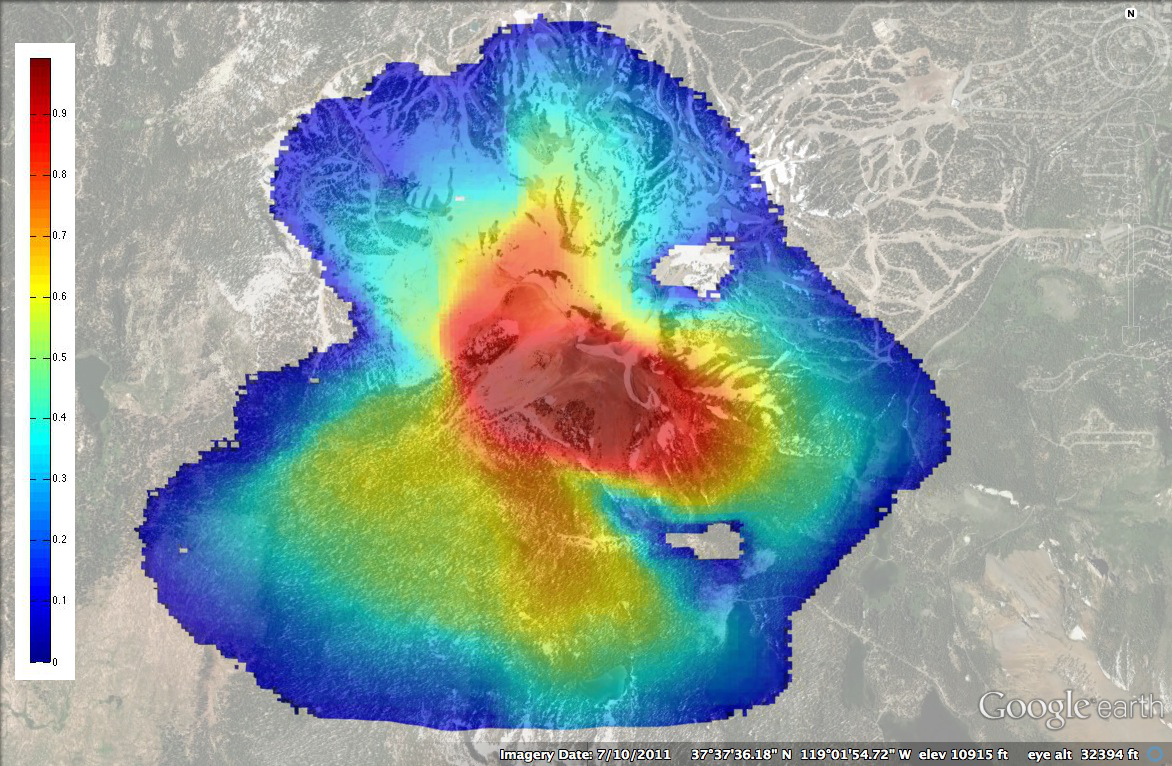
\includegraphics{mammoth.jpg}}%
\caption{\label{fig2} Figure shows the probabilistic hazard map (right) of the region around "Mammoth" volcano, 
for flow exceeding 0.2m of depth using 1024 samples generated with the above computing model.
}
\label{map2}
\end{center}
\end{figure}
\end{comment}
%%%%%%%%%%%%%%%%%%%%%%%%%%%%%%%% END  OF COMMENTS  %%%%%%%%%%%%%%%%%%%%%%%%%%%%%%%%%%%%%%%%%%%%%%%%%%%%%%%%%%%%%%%%%%



\section{CONCLUSION}
%The primary contribution of 
Through this paper is we aim to address the simultaneous computational and data challenges in a Uncertainty quantification process
%using a combination of algorithmic (localization and parallelization) and hardware approaches.
through two different approaches - one hardware based and other using a more popular software tool on the traditional cluster.
%An integrated workflow was successfully architected, 
We successfully architected and implemented two functional workflows for the application of generating hazard maps for geophysical flows.
Netezza based workflow offered a faster implementation for a moderate sized data such as ours in comparison to Hadoop based workflow.
Data mining tasks required minimal work
and its ability to perform fast analytics provided quick insight about the data. On the other hand, Netezza is an expensive hardware, with its
SPUs (Snippet Processing Units) prone to wearing out. Integrating Netezza with the cluster presented numerous hurdles and the
resulting implementation was not fault tolerant. Furthermore, restriction on the  number of 'working' ports on Netezza makes the workflow less
scalable. Hadoop in contrast is a much cheaper alternative, offering reliable and robust job scheduler and fault tolerance. It made our
implementation of the workflow programatically easy and obviated the need to move data from the cluster. It is also more easily scalable.
However, modeling, a compute intensive
task, such as emulator construction, as a mapper posed a severe problem. Using Hadoop API for tasks deficient in input data but requiring more cpu
cycles clearly suggested that it can't be used as an alternative job scheduler for compute intensive tasks.


\begin{comment}
A number of fundamental changes in the design of hazard map generation were introduced and were largely possible through the use of
Netezza server. 




With Netezza's data mining capability, tessellation based covariance localization \cite{keith,ramona} was completely replaced with a more  reliable distance based search for neighbors.
This not only leads to a more precise control of the region of neighborhood but also makes it more feasible to extend the problem to higher
dimensions. In addition search distance for each dimension can be separately incorporated making this model even more versatile.
The tessellation based method is firmly dependent on the manner in which spatial points are downsized making $\it{downsampling}$ a cornerstone in 
the process emulator construction. The workflow proposed in this paper attributes less importance to $\it{downsampling}$ 
and offers more flexibility than the previous approach.\\

It was also comparatively easier to work on a combination of Netezza server and the high performance cluster. The codes were more concise and
amenable to changes. Most importantly, information was communicated in a more elegant fashion, with very little need for
file handling. Data was pre-dominantly transferred over the network obviating the need to read and write large number of ASCII files.
Finally, this model is easily extended to a wide range of problems with 
the similar challenges of massive data movement and complex computations.
\end{comment}




\bibliographystyle{plain}
\bibliography{list}

\end{document}

















%%%%%%%%%%%%%%%%%%%%%%%%%%%%%%%%%%%%%%%%%%%%%%%%%     DO NOT BOTHER READING THIS ALL COMMNETED %%%%%%%%%%%%%%%%%%%%%%%%%%%%
\begin{comment}
\section{The {\secit Body} of The Paper}
Typically, the body of a paper is organized
into a hierarchical structure, with numbered or unnumbered
headings for sections, subsections, sub-subsections, and even
smaller sections.  The command \texttt{{\char'134}section} that
precedes this paragraph is part of such a
hierarchy.\footnote{This is the second footnote.  It
starts a series of three footnotes that add nothing
informational, but just give an idea of how footnotes work
and look. It is a wordy one, just so you see
how a longish one plays out.} \LaTeX\ handles the numbering
and placement of these headings for you, when you use
the appropriate heading commands around the titles
of the headings.  If you want a sub-subsection or
smaller part to be unnumbered in your output, simply append an
asterisk to the command name.  Examples of both
numbered and unnumbered headings will appear throughout the
balance of this sample document.

Because the entire article is contained in
the \textbf{document} environment, you can indicate the
start of a new paragraph with a blank line in your
input file; that is why this sentence forms a separate paragraph.

\subsection{Type Changes and {\subsecit Special} Characters}
We have already seen several typeface changes in this sample.  You
can indicate italicized words or phrases in your text with
the command \texttt{{\char'134}textit}; emboldening with the
command \texttt{{\char'134}textbf}
and typewriter-style (for instance, for computer code) with
\texttt{{\char'134}texttt}.  But remember, you do not
have to indicate typestyle changes when such changes are
part of the \textit{structural} elements of your
article; for instance, the heading of this subsection will
be in a sans serif\footnote{A third footnote, here.
Let's make this a rather short one to
see how it looks.} typeface, but that is handled by the
document class file. Take care with the use
of\footnote{A fourth, and last, footnote.}
the curly braces in typeface changes; they mark
the beginning and end of
the text that is to be in the different typeface.

You can use whatever symbols, accented characters, or
non-English characters you need anywhere in your document;
you can find a complete list of what is
available in the \textit{\LaTeX\
User's Guide}\cite{Lamport:LaTeX}.

\subsection{Math Equations}
You may want to display math equations in three distinct styles:
inline, numbered or non-numbered display.  Each of
the three are discussed in the next sections.

\subsubsection{Inline (In-text) Equations}
A formula that appears in the running text is called an
inline or in-text formula.  It is produced by the
\textbf{math} environment, which can be
invoked with the usual \texttt{{\char'134}begin. . .{\char'134}end}
construction or with the short form \texttt{\$. . .\$}. You
can use any of the symbols and structures,
from $\alpha$ to $\omega$, available in
\LaTeX\cite{Lamport:LaTeX}; this section will simply show a
few examples of in-text equations in context. Notice how
this equation: \begin{math}\lim_{n\rightarrow \infty}x=0\end{math},
set here in in-line math style, looks slightly different when
set in display style.  (See next section).

\subsubsection{Display Equations}
A numbered display equation -- one set off by vertical space
from the text and centered horizontally -- is produced
by the \textbf{equation} environment. An unnumbered display
equation is produced by the \textbf{displaymath} environment.

Again, in either environment, you can use any of the symbols
and structures available in \LaTeX; this section will just
give a couple of examples of display equations in context.
First, consider the equation, shown as an inline equation above:
\begin{equation}\lim_{n\rightarrow \infty}x=0\end{equation}
Notice how it is formatted somewhat differently in
the \textbf{displaymath}
environment.  Now, we'll enter an unnumbered equation:
\begin{displaymath}\sum_{i=0}^{\infty} x + 1\end{displaymath}
and follow it with another numbered equation:
\begin{equation}\sum_{i=0}^{\infty}x_i=\int_{0}^{\pi+2} f\end{equation}
just to demonstrate \LaTeX's able handling of numbering.

\subsection{Citations}
Citations to articles \cite{bowman:reasoning, clark:pct, braams:babel, herlihy:methodology},
conference
proceedings \cite{clark:pct} or books \cite{salas:calculus, Lamport:LaTeX} listed
in the Bibliography section of your
article will occur throughout the text of your article.
You should use BibTeX to automatically produce this bibliography;
you simply need to insert one of several citation commands with
a key of the item cited in the proper location in
the \texttt{.tex} file \cite{Lamport:LaTeX}.
The key is a short reference you invent to uniquely
identify each work; in this sample document, the key is
the first author's surname and a
word from the title.  This identifying key is included
with each item in the \texttt{.bib} file for your article.

The details of the construction of the \texttt{.bib} file
are beyond the scope of this sample document, but more
information can be found in the \textit{Author's Guide},
and exhaustive details in the \textit{\LaTeX\ User's
Guide}\cite{Lamport:LaTeX}.

This article shows only the plainest form
of the citation command, using \texttt{{\char'134}cite}.
This is what is stipulated in the SIGS style specifications.
No other citation format is endorsed.

\subsection{Tables}
Because tables cannot be split across pages, the best
placement for them is typically the top of the page
nearest their initial cite.  To
ensure this proper ``floating'' placement of tables, use the
environment \textbf{table} to enclose the table's contents and
the table caption.  The contents of the table itself must go
in the \textbf{tabular} environment, to
be aligned properly in rows and columns, with the desired
horizontal and vertical rules.  Again, detailed instructions
on \textbf{tabular} material
is found in the \textit{\LaTeX\ User's Guide}.

Immediately following this sentence is the point at which
Table 1 is included in the input file; compare the
placement of the table here with the table in the printed
dvi output of this document.

\begin{table}
\centering
\caption{Frequency of Special Characters}
\begin{tabular}{|c|c|l|} \hline
Non-English or Math&Frequency&Comments\\ \hline
\O & 1 in 1,000& For Swedish names\\ \hline
$\pi$ & 1 in 5& Common in math\\ \hline
\$ & 4 in 5 & Used in business\\ \hline
$\Psi^2_1$ & 1 in 40,000& Unexplained usage\\
\hline\end{tabular}
\end{table}

To set a wider table, which takes up the whole width of
the page's live area, use the environment
\textbf{table*} to enclose the table's contents and
the table caption.  As with a single-column table, this wide
table will ``float" to a location deemed more desirable.
Immediately following this sentence is the point at which
Table 2 is included in the input file; again, it is
instructive to compare the placement of the
table here with the table in the printed dvi
output of this document.


\begin{table*}
\centering
\caption{Some Typical Commands}
\begin{tabular}{|c|c|l|} \hline
Command&A Number&Comments\\ \hline
\texttt{{\char'134}alignauthor} & 100& Author alignment\\ \hline
\texttt{{\char'134}numberofauthors}& 200& Author enumeration\\ \hline
\texttt{{\char'134}table}& 300 & For tables\\ \hline
\texttt{{\char'134}table*}& 400& For wider tables\\ \hline\end{tabular}
\end{table*}
% end the environment with {table*}, NOTE not {table}!

\subsection{Figures}
Like tables, figures cannot be split across pages; the
best placement for them
is typically the top or the bottom of the page nearest
their initial cite.  To ensure this proper ``floating'' placement
of figures, use the environment
\textbf{figure} to enclose the figure and its caption.

This sample document contains examples of \textbf{.eps}
and \textbf{.ps} files to be displayable with \LaTeX.  More
details on each of these is found in the \textit{Author's Guide}.

\begin{figure}
\centering
\epsfig{file=fly.eps}
\caption{A sample black and white graphic (.eps format).}
\end{figure}

\begin{figure}
\centering
\epsfig{file=fly.eps, height=1in, width=1in}
\caption{A sample black and white graphic (.eps format)
that has been resized with the \texttt{epsfig} command.}
\end{figure}


As was the case with tables, you may want a figure
that spans two columns.  To do this, and still to
ensure proper ``floating'' placement of tables, use the environment
\textbf{figure*} to enclose the figure and its caption.

Note that either {\textbf{.ps}} or {\textbf{.eps}} formats are
used; use
the \texttt{{\char'134}epsfig} or \texttt{{\char'134}psfig}
commands as appropriate for the different file types.

\subsection{Theorem-like Constructs}
Other common constructs that may occur in your article are
the forms for logical constructs like theorems, axioms,
corollaries and proofs.  There are
two forms, one produced by the
command \texttt{{\char'134}newtheorem} and the
other by the command \texttt{{\char'134}newdef}; perhaps
the clearest and easiest way to distinguish them is
to compare the two in the output of this sample document:

This uses the \textbf{theorem} environment, created by
the\linebreak\texttt{{\char'134}newtheorem} command:
\newtheorem{theorem}{Theorem}
\begin{theorem}
Let $f$ be continuous on $[a,b]$.  If $G$ is
an antiderivative for $f$ on $[a,b]$, then
\begin{displaymath}\int^b_af(t)dt = G(b) - G(a).\end{displaymath}
\end{theorem}

The other uses the \textbf{definition} environment, created
by the \texttt{{\char'134}newdef} command:
\newdef{definition}{Definition}
\begin{definition}
If $z$ is irrational, then by $e^z$ we mean the
unique number which has
logarithm $z$: \begin{displaymath}{\log e^z = z}\end{displaymath}
\end{definition}

\begin{figure}
\centering
\psfig{file=rosette.ps, height=1in, width=1in,}
\caption{A sample black and white graphic (.ps format) that has
been resized with the \texttt{psfig} command.}
\end{figure}

Two lists of constructs that use one of these
forms is given in the
\textit{Author's  Guidelines}.

\begin{figure*}
\centering
\epsfig{file=flies.eps}
\caption{A sample black and white graphic (.eps format)
that needs to span two columns of text.}
\end{figure*}
and don't forget to end the environment with
{figure*}, not {figure}!
 
There is one other similar construct environment, which is
already set up
for you; i.e. you must \textit{not} use
a \texttt{{\char'134}newdef} command to
create it: the \textbf{proof} environment.  Here
is a example of its use:
\begin{proof}
Suppose on the contrary there exists a real number $L$ such that
\begin{displaymath}
\lim_{x\rightarrow\infty} \frac{f(x)}{g(x)} = L.
\end{displaymath}
Then
\begin{displaymath}
l=\lim_{x\rightarrow c} f(x)
= \lim_{x\rightarrow c}
\left[ g{x} \cdot \frac{f(x)}{g(x)} \right ]
= \lim_{x\rightarrow c} g(x) \cdot \lim_{x\rightarrow c}
\frac{f(x)}{g(x)} = 0\cdot L = 0,
\end{displaymath}
which contradicts our assumption that $l\neq 0$.
\end{proof}

Complete rules about using these environments and using the
two different creation commands are in the
\textit{Author's Guide}; please consult it for more
detailed instructions.  If you need to use another construct,
not listed therein, which you want to have the same
formatting as the Theorem
or the Definition\cite{salas:calculus} shown above,
use the \texttt{{\char'134}newtheorem} or the
\texttt{{\char'134}newdef} command,
respectively, to create it.

\subsection*{A {\secit Caveat} for the \TeX\ Expert}
Because you have just been given permission to
use the \texttt{{\char'134}newdef} command to create a
new form, you might think you can
use \TeX's \texttt{{\char'134}def} to create a
new command: \textit{Please refrain from doing this!}
Remember that your \LaTeX\ source code is primarily intended
to create camera-ready copy, but may be converted
to other forms -- e.g. HTML. If you inadvertently omit
some or all of the \texttt{{\char'134}def}s recompilation will
be, to say the least, problematic.

\section{Conclusions}
This paragraph will end the body of this sample document.
Remember that you might still have Acknowledgments or
Appendices; brief samples of these
follow.  There is still the Bibliography to deal with; and
we will make a disclaimer about that here: with the exception
of the reference to the \LaTeX\ book, the citations in
this paper are to articles which have nothing to
do with the present subject and are used as
examples only.
%\end{document}  % This is where a 'short' article might terminate

%ACKNOWLEDGMENTS are optional
\section{Acknowledgments}
This section is optional; it is a location for you
to acknowledge grants, funding, editing assistance and
what have you.  In the present case, for example, the
authors would like to thank Gerald Murray of ACM for
his help in codifying this \textit{Author's Guide}
and the \textbf{.cls} and \textbf{.tex} files that it describes.

%
% The following two commands are all you need in the
% initial runs of your .tex file to
% produce the bibliography for the citations in your paper.
\bibliographystyle{abbrv}
\bibliography{sigproc}  % sigproc.bib is the name of the Bibliography in this case
% You must have a proper ".bib" file
%  and remember to run:
% latex bibtex latex latex
% to resolve all references
%
% ACM needs 'a single self-contained file'!
%
%APPENDICES are optional
%\balancecolumns
\appendix
%Appendix A
\section{Headings in Appendices}
The rules about hierarchical headings discussed above for
the body of the article are different in the appendices.
In the \textbf{appendix} environment, the command
\textbf{section} is used to
indicate the start of each Appendix, with alphabetic order
designation (i.e. the first is A, the second B, etc.) and
a title (if you include one).  So, if you need
hierarchical structure
\textit{within} an Appendix, start with \textbf{subsection} as the
highest level. Here is an outline of the body of this
document in Appendix-appropriate form:
\subsection{Introduction}
\subsection{The Body of the Paper}
\subsubsection{Type Changes and  Special Characters}
\subsubsection{Math Equations}
\paragraph{Inline (In-text) Equations}
\paragraph{Display Equations}
\subsubsection{Citations}
\subsubsection{Tables}
\subsubsection{Figures}
\subsubsection{Theorem-like Constructs}
\subsubsection*{A Caveat for the \TeX\ Expert}
\subsection{Conclusions}
\subsection{Acknowledgments}
%\subsection{Additional Authors}
This section is inserted by \LaTeX; you do not insert it.
You just add the names and information in the
\texttt{{\char'134}additionalauthors} command at the start
of the document.
\subsection{References}
Generated by bibtex from your ~.bib file.  Run latex,
then bibtex, then latex twice (to resolve references)
to create the ~.bbl file.  Insert that ~.bbl file into
the .tex source file and comment out
the command \texttt{{\char'134}thebibliography}.
% This next section command marks the start of
% Appendix B, and does not continue the present hierarchy
\section{More Help for the Hardy}
The acm\_proc\_article-sp document class file itself is chock-full of succinct
and helpful comments.  If you consider yourself a moderately
experienced to expert user of \LaTeX, you may find reading
it useful but please remember not to change it.
\balancecolumns
% That's all folks!
\end{comment}

%%%%%%%%%%%%%%%%%%%%%%%%%%%%%%%%%%%%%%%%%% END OF DO NOT BOTHER READING COMMENTS   %%%%%%%%%%%%%%%%%%%%%%%%%%%%%%%%%%%%%


\bibliographystyle{plain}
\bibliography{list}

\end{document}
